\section{ANSE testbed}

A typical PhEDEx installation consists of:
\begin{itemize}
	\item central agents
	\item site agents
	\item central Oracle database
	\item one or more front-ends \\
\end{itemize}

In the context of the ANSE project, the central agents, DB and frontend all run
at CERN. The site agents are running on machines located in different geographical
locations. (see Figure \ref{fig:ANSE-setup}).

\begin{figure}[h]
  \centering
  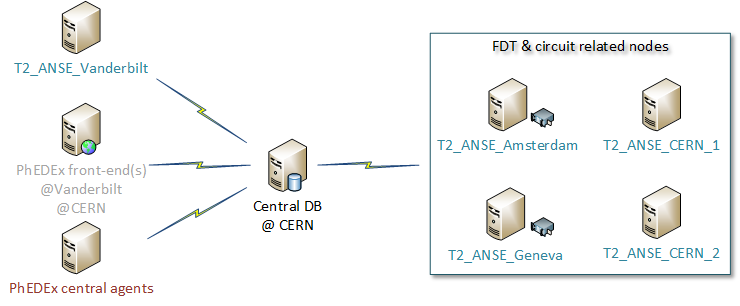
\includegraphics[width=0.95\textwidth]{Figures/ANSE-setup.png}
  \caption{PhEDEx setup for ANSE}
  \label{fig:ANSE-setup}
\end{figure}

For development work and prototype tests we mainly use OpenStack virtual machines.
These contain PhEDEx installations and also double as small storage nodes. These
typically have 8GB of RAM, 4 VCPUs and 80GB disk. These VMs are able to have
sustained disk-to-disk transfer rates of 1Gbps.

For more advanced tests we use four physical servers, two located in Geneva and 
two in Amsterdam. In each location, one of the two servers is used as a PhEDEx node, 
while the other is used a storage node.

Each storage node (sandy01-gva and sandy01-ams) has dual E5-2670 CPUs (32 logical cores)
64GB or RAM and 2 LSI disk controllers. Each of the LSI controllers manages
8 high speed SSDs. Two RAID-0 arrays are created on each LSI controller (4 SSD per
RAID 0 array).

Between the two storage nodes we have a high capacity 40Gbps link and use Ciena
routers to create dynamic links between them.

Since the storage nodes were designed for high speed rather than high capacity,
we created a large number of soft links to large random-filled files (2->15GB) 
on the source disk. 

On the destination side we either used a crontab running every minute to remove
transferred files, or we relied on the PhEDEx post-validation  script to remove 
files in bulk at the end of a transfer job.

Monitoring is performed with MonALISA\cite{MonALISA} and PhEDEx.
